\chapter{Systemy rekomendacji}
\thispagestyle{chapterBeginStyle}

\section{Rodzaje systemów rekomendacji}

Systemy rekomendacji to rodzaj filtrów informacji, które powstały w celu odnalezienia w zbiorze danych produktu, który trafi w osobiste preferencje użytkownika. Występują one w całym Internecie rozpowszechnione za sprawą wyszukiwarek internetowych, dla których początkowo powstały. Jednym z pierwszych takich miejsc, w którym możemy się na nie natknąć pojawia się przy okazji autouzupełniania (ang. \textit{autocomplete}) wpisywanego tekstu. Naturalne stało się to, że nowoczesne narzędzia tworzą dla nas podpowiedzi, co dzieje się na podstawie częstotliwości wpisanych fraz przez innych użytkowników oraz historii naszych wcześniejszych wyszukań. W ten sposób pomagają one uniknąć takich pomyłek jak błędy ortograficzne czy literówki. Dodatkowo, zastosowanie takiego mechanizmu w wyszukiwarce internetowej ułatwia jej udzielenie poprawnej odpowiedzi na stworzone zapytanie, poprzez zaproponowanie specjalistycznego słownictwa lub synonimu, który lepiej pasuje w danym kontekście. Przechodząc do wyszukiwarek natrafiamy na kolejny przykład wykorzystania naszych systemów, a mianowicie globalne systemy rankingowe, czyli sposób na ocenę i pozycjonowanie wszystkich stron internetowych w wynikach wyszukiwania. Idea działania algorytmu PageRank (wykorzystanego m.in. w przeglądarce Google) została opisana w dalszej części pracy, w rozdziale poświęconemu temu zagadnieniu.

Zastosowaniem, na którym skupiamy się w tej pracy jest personalizacja wyników pod konkretnych użytkowników (w skrócie PRES, z ang. \textit{Personalized Recommender System}). Takie silniki rekomendacji znajdują swoje zastosowanie głównie w komercyjnych rozwiązaniach, gdzie odpowiednia propozycja może w znaczący sposób zachęcić użytkownika do ponownego skorzystania z serwisu. Najpopularniejsze aplikacje tych systemów to generowanie playlist dla serwisów wideo oraz muzyki jak Youtube i Netflix, tworzenie preferencyjnych ofert dla użytkowników aukcji internetowych takich jak Amazon czy Allegro lub tworzenie dla portali społecznościowych jak Facebook czy Twitter powiązań między użytkownikami. Ze względu na różnice w implementacji możemy rozpatrzyć 3 różne podejścia:
\begin{itemize}
    \item metoda content-based,
    \item metoda collaborative filtering,
    \item metoda hybrydowa, która łączy dwie pierwsze podejścia.
\end{itemize}

\begin{figure}[h]
    \centering
    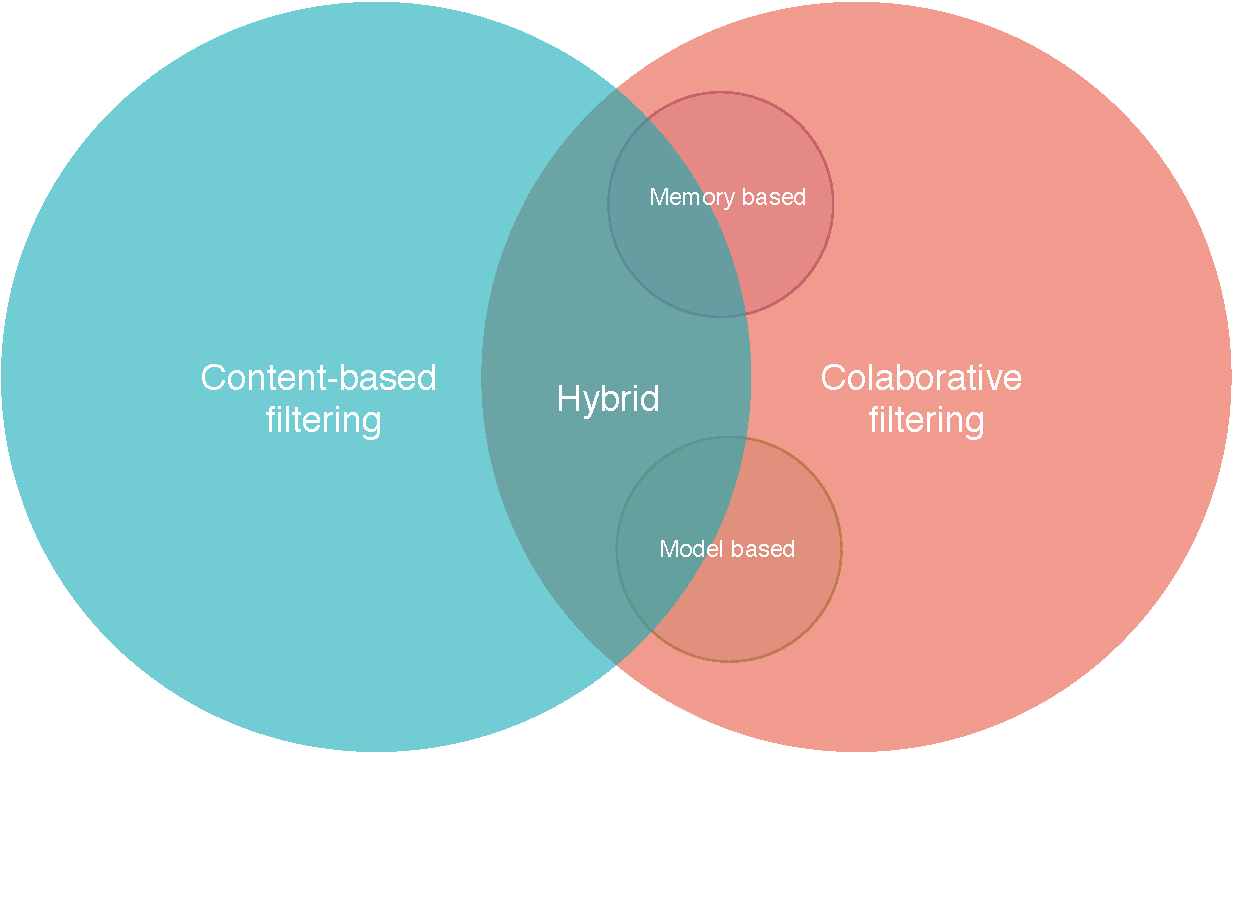
\includegraphics[width=\textwidth]{data/Venn.pdf}
    \caption{Podział systemów rekomendacji}
    \label{fig:my_label}
\end{figure}

\section{Gromadzenie informacji}

Zanim przejdziemy do opisu metod tworzenia rankingu, musimy w jakiś sposób zebrać dane o użytkowniku, aby poznać jego preferencje. W tym celu zasadniczo korzysta się dwóch źródeł informacji, z jawnej (ang. explicit feedback) lub domniemanej  (ang. implicit feedback) informacji zwrotnej. Pierwszą uzyskujemy poprzez przeprowadzenie ankiety na nowo stworzonym koncie w celu bezpośredniego uzupełnienia informacji o interesujących nas cechach na podstawie odpowiedzi jakie zostały udzielone. Tak uzyskane informacje mogą pozytywnie wpłynąć na modelowanie użytkownika oraz generowanie rekomendacji:
\begin{itemize}
    \item Po pierwsze pomagają w rozwiązaniu problemu braku gęstości danych (ang. \textit{large data sparesity}) poprzez wymuszenie dodatkowych informacji o preferencjach użytkownika, a co za tym idzie zwiększenie liczby relacji między obiektami w systemie.
    \item Po drugie rozwiązuje cold-start problem, na który napotykamy w systemach rekomendacji w momencie, gdy rejestruje się nowy użytkownik i nie mamy o nim żadnych informacji. W tym problemie rozróżniamy dwa rodzaje użytkowników: pierwszy, który miał małą styczność z obiektami w systemie oraz drugi, który jest całkowicie nowy dla systemu. Dla pierwszego typu ankieta może zostać wykorzystana do wzmocnienia oceny atrybutów w profilu użytkownika, a dla drugiego do stworzenia takiego profilu oraz polepszenia jakości całego rankingu.
    \item Trzecią korzyścią płynąca z zastosowania ankietyzacja użytkowników dla modeli, które nie mierzą się z problemem małej ilości danych jest ustalenie jakości stworzonego rankingu poprzez porównanie go z odpowiedziami udzielonymi w ankiecie oraz rozpoznanie ukrytych preferencji użytkownika, które nie zostały wykryte innymi metodami. \cite{RecommenderSystemsBasedonUserReviews:TheStateoftheArt}
\end{itemize}

Portale na których pobierana jest informacja od użytkownika (np. Twitter oraz Pintrest) czerpią ogromne korzyści z możliwości wyświetlania dostosowanej do niego zawartości. 
Zaraz po rejestracji użytkownik proszony jest o ocenę jakie treści go interesują w celu zapewnienia spersonalizowanych rekomendacji. W ten sposób, o ile ankietowany nie skłamał w odpowiedziach, możemy zaprezentować mu treści pasujące do jego upodobań.

Drugim rozwiązaniem jest wykorzystanie wcześniejszych zachowań lub wyborów użytkownika. Można wykorzystać np. wcześniej wybrany przez niego przedmiot lub czas jaki spędzi podczas przeglądania oferty. Zbieraniem informacji o jego działaniach zajmuje się system, który monitoruje każdy jego ruch. Implementacja tego podejścia jest o wiele bardziej skomplikowana, dlaczego często łączona jest z pierwszą, na przykład w serwisie YouTube przy rekomendacji filmów wykorzystywana jest informacja jawna o tym które kanały zostały przez użytkownika zasubskrybowane i polubione, oraz dodatkowo zbierane są informacje o tym, które filmy zostały przez niego obejrzane w całości, a z oglądania których zrezygnował po kilku minutach.

Popularną metodą wykorzystywaną do wydobycia ważnych z punktu widzenia systemu informacji o użytkowniku bez jego aktywnego zaangażowania, używany w 83\% biblotek cyfrowych \cite{Research-paperrecommendersystems:aliteraturesurvey} jest indeks \textit{tf-idf} (ang. term frequency–inverse document frequency). Tradycyjnie wykorzystany jest on do analizy dokumentów tekstowych i umożliwia wskazanie słów najbardziej charakterystycznych dla danego dokumentu, w kontekście większego zbioru dokumentów. Jego pierwszym krokiem jest pozbycie z dokumentów tagów oraz słów, które nie zapewniają istotnych informacji np. znaków interpunkcyjnych oraz często występujących słów. Kolejno z pozostałego zbioru usuwane są prefisy i sufixy w celu odnalezienia podstawowej formy słowa. Następnie bazując na tym jak użytkownik ocenił treść (jawny lub bierny sposób uzyskiwania informacji o preferencjach użytkownika) wybieramy te słowa (termy), które są z punktu widzenia użytkownika interesujące wykorzystując w tym celu wzór na wartość tf-idf:
\begin{equation}
\label{tfidf}
        \mathrm{(tf\text{-}idf)_{i,j}} = \mathrm{tf_{i,j}} \times \mathrm{idf_i},
\end{equation}
gdzie:
\begin{itemize}
    \item $tf_{i, j}$to tzw. „term frequency”, wyrażana wzorem:
\end{itemize}
\begin{equation*}
    \mathrm{tf_{i,j}} = \frac{n_{i,j}}{\sum_k n_{k,j}},
\end{equation*}
gdzie: 
\begin{itemize}
    \item $n_{i,j}$ jest liczbą wystąpień termu $(t_i)$ w dokumencie $d_j,$ a mianownik jest sumą liczby wystąpień wszystkich termów w dokumencie $d_j.$
    \item $idf_{i}$ to „inverse document frequency” wyrażana wzorem:
\end{itemize}
\begin{equation*}
    \mathrm{idf_i} = \log \frac{|D|}{|\{d: t_i \in d\}|},
\end{equation*}
gdzie:
\begin{itemize}
    \item $|D|$ – liczba dokumentów w korpusie,
    \item $|\{d : t_i \in d\}|$ – liczba dokumentów zawierających przynajmniej jedno wystąpienie danego termu.

\end{itemize}

\section{Content-based filtering}
\label{chap:content}


Metoda content-based filtering (CB) rekomenduje użytkownikowi produkty na podstawie utworzonego profilu użytkownika. To podejście najlepiej sprawdza się w sytuacji, gdy znamy dokładne informacje o produkcie (nazwa, lokalizacja, opis), ale mamy niewiele informacji o użytkowniku.

Na początku zarówno dla przedmiotów jak i użytkowników tworzymy profil, typowo reprezentowany za pomocą wektora $X=(x_{1},x_{2},...,x_{n})$, gdzie $x_{n}$ reprezentuje pewną cechę lub atrybut. Następnie porównując wektory za pomocą różnych metryk, możemy obliczyć odległości między nimi i stworzyć ranking, który pozwoli na wybranie przedmiotów podobnych do wektora użytkownika. W rezultacie otrzymujemy listę przedmiotów, które powinny pokryć się z upodobaniami użytkownika.

Jedną z takich miar używanych w przypadku, kiedy rozpatrywane wektory są binarne (wektor składa się z samych zer i jedynek) jest odległość Hamminga. Jej wartość dla dwóch ciągów tej samej długości to liczba pozycji, na których ciągi mają różne wartości. 
W przypadku, gdy wektory składają się z liczb rzeczywistych typowo wykorzystuje się odległość euklidesową \cite{Similarityandrecommendersystems}.
Jeśli w kartezjańskim układzie współrzędnych $\mathbf{a}=(a_1,a_2,...,a_n)$ i $\mathbf{b}=(b_1,b_2,...,b_n)$ są dwoma punktami w n-wymiarowej przestrzeni euklidesowej to odległość (d) między $\mathbf{a}$ i $\mathbf{b}$ lub $\mathbf{b}$ i $\mathbf{a}$ wynosi:
\begin{equation}
    \begin{aligned}
        d(\mathbf{a},\mathbf{b}) = d(\mathbf{a},\mathbf{b}) & = \sqrt{(a_1-b_1)^2 + (a_2-b_2)^2 + \cdots + (a_n-b_n)^2} \\
& = \sqrt{\sum_{i=1}^n (a_i-b_i)^2}.
    \end{aligned}
\end{equation}

Zauważmy w tym miejscu dodatkowo, że w przypadku porównania przedmiotów (ang. \textit{item-to-item}) najczęściej wykorzystywana jest jedna z dwóch następujących miar odległości:
\begin{itemize}
    \item odległość kosinusowa, czyli kosinus kąta między dwoma wektorami reprezentującymi dwóch użytkowników lub dwa produkt \cite{Eksploracjatekstu}. Jego wartość $\cos(\theta)$ obliczana jest następująco:
    \begin{equation}
        \cos(\theta) = {\mathbf{a} \cdot \mathbf{b} \over \|\mathbf{a}\| \|\mathbf{b}\|} = \frac{ \sum\limits_{i=1}^{n}{a_i  b_i} }{ \sqrt{\sum\limits_{i=1}^{n}{a_i^2}}  \sqrt{\sum\limits_{i=1}^{n}{b_i^2}} }~.
    \end{equation}
    Wykorzystywana jest ona między innymi w sklepie internetowym Amazon \cite{Amazon.comRecommendationsItem-to-ItemCollaborativeFiltering}.
    \item Indeks Jaccarda, zdefiniowany jako moc części wspólnej zbiorów $A$ i $B$ przez moc ich sumy, mierzy podobieństwo pomiędzy dwoma zbiorami:
    \begin{equation}
       J (A,B) = \frac{|A \cap B|}{|A \cup B|}.
    \end{equation}
    Podobnie jak odległość Hamminga współczynnik podobieństwa Jaccarda znajduje swoje zastosowanie w systemach rekomendacji w sytuacji, gdy wektory reprezentowane są poprzez wartości binarne.
\end{itemize}

Dzięki zastosowaniu jednej z powyżej opisanych miar odległości jesteśmy w stanie ustalić odległość między wektorami. Jednakże, aby dane były gotowe do porównania i analizy, często wymagają dodatkowych zabiegów. Dla przykładu rozważmy system rekomendacji do rekomendacji filmów i dwóch użytkowników tego systemu, z których jeden konsekwentnie ocenia wyżej niż drugi (zawyża oceny). Odległość między tymi użytkownikami może być duża. Z tego powodu 
typowo stosuję się normalizację ocen, doprowadzając wektory do tzw. postaci standardowej \cite{Similarityandrecommendersystems}.
Niech wektor $x_u = (x_{u1}, x_{u2}, ... , x_{uN})$ opisuje użytkownika $u$, gdzie $x_{un}$ jest jego oceną produktu $n$. Obliczamy średnią ocenę $\overline{x}_{u}$ oraz odchylenie standardowe $s_{u}$ w następujący sposób:
\begin{equation}
\label{eqn:normalizacja1}
     \overline{x}_{u} = \frac{1}{N}\sum_{n=1}^N x_{un}~,
\end{equation}
\begin{equation}
\label{eqn:normalizacja2}
    s_{u} = \sqrt{\frac{1}{N-1} \sum_{n=1}^N(x_{un} - \overline{x}_{u})^2}~.
\end{equation}
Następnie zmieniamy zmienną niestandaryzowaną $x_{un}$ na:
\begin{equation}
\label{eqn:normalizacja3}
    z_{un}= \frac{x_{un}-\overline{x}_{u}}{s_{u}}~.
\end{equation}

System rekomendacji oparty na technice content-based filtering, po obliczeniu podobieństwa pomiędzy przedmiotami a użytkownikami tworzy listę najlepszych rekomendacji. Jeśli niepożądane jest, aby użytkownikowi został polecany produkt, który jest mu już znany, systemu usuwa te pozycje, a następnie prezentuje wynik użytkownikowi. Wadą content-based filtering jest potrzeba wydobycia charakterystycznych cech z przedmiotu, co nie zawsze jest łatwe lub wykonalne. Jeśli przedmiot posiada opis tekstowy, z którego możemy uzyskać informacje
(na przykład wykorzystując indeks tf-idf), wtedy metoda content-based zadziała. Jednakże problem napotykamy w np. momencie w przypadku prób rekomendacji muzyki lub obrazu, gdyż najczęściej nie istnieje łatwy sposób na stworzenie ich matematycznej reprezentacji.

\section{Collaborative filtering}

Druga z technik stosowanych w systemach rekomendacji to collaborative filtering (CF). Bazuje ona na pomyśle, że użytkownikom o podobnych upodobaniach odpowiadają podobne produkty. W tym przypadku nie wykorzystujemy charakterystyki produktów, upodobania użytkownika są określane na podstawie jego historii z produktami np. jakie produkty kupił, a następnie na tej podstawie obliczane są korelacje między użytkownikami. Następnie te korelacje służą do stworzenia dopasowania produktów dla konkretnego użytkownika.

Wśród algorytmów rekomendacji wykorzystujących collaborative filtering wyróżniamy 2 podgrupy:
\begin{itemize}
    \item metody wykorzystujące pamięć,
    \item metody wykorzystując model.
\end{itemize}

\subsection{Metody wykorzystujące pamięć}
W metodach wykorzystujące pamięć ponownie można wydzielić 2 typy ze względu na to jakie dane przetwarzają: filtracja użytkownik-produkt (ang. \textit{user-item filtering}) oraz filtracja produkt-produkt (ang.\textit{item-item filtering}).
Przykładem aplikacji filtracji użytkownik-produkt jest algorytm klasyfikacji K najbliższych sąsiadów, który znajduje grupy użytkowników o podobnych zainteresowaniach. Przepływ pracy w tym przypadku standardowo przebiega w 3 krokach:
\begin{itemize}
    \item Użytkownik ocenia dany produkt. Może to się dokonać tak samo jak w poprzedniej metodzie w sposób jawny (ang. \textit{explicit feedback}) lub bierny (ang. \textit{implicit feedback}). Pierwszy polega na bezpośredniej ocenie produktu przez uzytkownika, a drugi na analizie jego zachowań.
    \item System porównuje ocenę produktów użytkownika z oceną innych użytkowników i na tej podstawie wyszukuje tych, którzy mają podobne upodobania jak ten dla którego tworzymy rekomendacje.
    \item Na końcu system rekomenduje przedmioty, które użytkownicy o podobnym guście ocenili wysoko, lecz nie zostały one jeszcze ocenione przez tego użytkownika.
\end{itemize}


Z kolei w przypadku filtracji produkt-produkt cały proces przebiega w następujący sposób:


\begin{itemize}
    \item Ocena produktów przez użytkownika przebiega identycznie jak w filtracji użytkownik-produkt,
    \item Utworzona zostaje macierz reprezentująca relacje między każdą parą przedmiotów.
    \item Na końcu system na wyszukuje w macierzy te przedmioty, które podobały sie użytkownikowi, na tej podstawie odszukuje tych użytkowników, których lubili te przedmioty i zwraca inne produkty, które lubili.
\end{itemize}
Podsumowując w pierwszym przypadku dane wejściowe to użytkownicy, a dane wyjściowe to produkty, a w drugim zarówno dane wejściowe jak i wyjściowe stanowią produkty. W skrócie filtracja użytkownik-produkt może zostać opisana jako “Użytkownikom podobnym do ciebie również podobało się...”, a filtracja produkt-produkt “Użytkownicy, którzy polubili ten produkt również polubili...”.

Podobnie jak przy metodzie content-based, podobieństwo obliczane jest za pomocą odpowiednich miar. Do tego celu wykorzystywana jest opisana już wcześniej odległość kosinusowa lub bardziej popularny w przypadku collaborative filtering współczynnik korelacji Pearsona. Do oszacowania korelacji między ocenami po pierwsze normalizujemy je przy korzystaniu wzorów \eqref{eqn:normalizacja1}, \eqref{eqn:normalizacja2} i \eqref{eqn:normalizacja3} do postaci standardowej, następnie obliczamy korelacje miedzy użytkownikami $x$ i $y$ według następującego wzoru:
\begin{equation}
\begin{aligned}
        r_{xy} & =\frac{1}{N-1} \sum ^N _{n=1} \left( \frac{x_n - \bar{x}}{s_x} \right) \left( \frac{y_n - \bar{y}}{s_y} \right) \\
        & = \frac{1}{N-1} \sum ^N _{i=n} z_{xn} z_{yn}
\end{aligned}
\end{equation}
gdzie:
\begin{itemize}
    \item N - wymiar wektora $x$ oraz $y$,
    \item $x_u = (x_{u1}, x_{u2}, ... , x_{uN})$, opisuje użytkownika $u$, gdzie $x_{un}$ jest oceną produktu n, analogicznie dla $y$,
    \item $\overline{x}$, $\overline{y}$ - średnia dla próby,
    \item $s_x$, $s_y$ - odchylenie standardowe.
\end{itemize}

Korelację można interpretować w następujący sposób: jeśli $z_{xn}$ jest duże, gdy $z_{yn}$ jest duże oraz, gdy $z_{xn}$ jest małe, gdy $z_{yn}$ jest małe wynik korelacji będzie zmierzał do $1$. Jeśli  $z_{xn}$ jest duże, gdy $z_{yn}$ jest małe oraz, gdy $z_{xn}$ jest duże, gdy $z_{yn}$ jest małe wynik korelacji będzie zmierzał do $-1$. W przypadku braku korelacji między użytkownikami wynik korelacji wynik będzie zmierzał do $0$ \cite{Similarityandrecommendersystems}.

\subsection{Metody wykorzystujące model}
Drugie podejście (ang. \textit{model-based collaborative filtering}) polega na stworzeniu rankingu w oparciu o pewien wybrany model.
Przy wykorzystaniu collaborative filtering napotykamy na różnego rodzaju problemy, których kilka opisujemy poniżej.   
Najistotniejsze problemy to brak gęstości danych (ang. data sparsity) i problem skalowalności, które wynikają z tego, że większość komercyjnych systemów rekomendacji jest oparta na wielkich bazach danych. Przez to macierze opisujące relacje między użytkownikiem a produktami i czas wykonywania operacji na takich macierzach rosną do bardzo dużych rozmiarów. Dla przykładu, w serwisie Twitter stosowane są techniki redukcji nieistotnych połączeń oraz dzielenie użytkowników na wiele grup dzięki czemu możliwe jest zastosowanie architektury umożliwiającej  wykonanie obliczeń w klastrze (trwają one wiele miesięcy)  \cite{WTF:TheWhotoFollowServiceatTwitter}.
W takich scenariuszach stosuje się techniki takie jak naiwny klasyfikator bayesowski, analiza skupień (ang. clustering models), przetwarzanie języka naturalnego (ang. \textit{latent semantic analysis}) czy też procesy decyzje Markowa.


Kolejny problem związany z brakiem gęstości danych jest tzw. zimny start (ang. \textit{cold start}). Napotykamy na niego w momencie pojawienia się w systemie nowego użytkownika lub produktu. Taki użytkownik, który nie ocenił produktów lub nowy produkt który nie został jeszcze oceniony wystarczającą ilość razy nie może być odpowiednio wdrożony do systemu. 
Tego rodzaju obiekt nazywa jest ,,czarną owcą'', gdy niemożliwe jest dopasowanie rekomendacji lub ,,szarą owcą'', gdy rekomendacje dla danego obiektu nie są konsekwentne. Ponieważ ten problem nie pojawia się w podejściu content-based  (w której mamy dostępny wektor ustalonych cech) często łączy się obie metody. Takie hybrydowe podejście nazywa się content-boosted collaborative filtering. 

Kolejnym wyzwaniem jest problem długiego ogona (ang. \textit{long tail}), który pojawia się w przypadku gdy większość użytkowników otrzymuje jako rekomendacje, tylko nieznaczna ilość przedmiotów w systemie.

\begin{figure}[h]
    \centering
    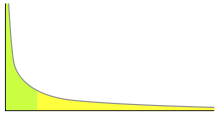
\includegraphics[width=0.4\textwidth]{longtail.png}
    \caption{Zobrazowanie problemu długiego ogona (źródło: \cite{WikipediaEN:Longtail}). Po prawej (żółty kolor) znajduje się długi ogon, po lewej (zielony kolor) reprezentuje małą grupę produktów, które dominują w rekomendacjach.}
    \label{fig:longtail}
\end{figure}


\section{Spacery losowe}
\label{chap:spacerylosowe}

System rekomendacji zaproponowany w tej pracy oparty jest na spacerach losowych. Poniżej przypominamy pojęcia związane ze spacerami losowymi zaczynając od pojęcia procesu stochastycznego i łańcucha Markowa. Proces stochastyczny definiujemy jako rodzinę zmiennych losowych $\mathbf{X}=\{X(t): t \in T\}$. Oznaczenie $X(t)$ lub $X_t$ rozumiemy jako stan procesu w czasie $t$. 
Będziemy dalej rozpatrywać procesy z czasem dyskretnym i skończone (tzn. zmienne $X_t$ będą przyjmować wartości ze zbioru skończonego). Łańcuch Markowa definiujemy następująco:

\begin{definition}\label{def:markow}
Jednorodny proces stochastyczny z czasem dyskretnym $X_{0}, X_{1}, X_{2},\dots$ jest łańcuchem Markowa, jeśli \cite{Metodyksiazka}

\begin{equation}
\begin{aligned}
    Pr(X_{t}= a_{t} | X_{t-1} = a_{t-1}, X_{t-2} = a_{t-2},\dots, X_{0} = a_{0}) = & Pr(X_{t} = a_{t} | X_{t-1} = a_{t-1}) = \\ & P_{a_{t-1},a_{t}} .
\end{aligned}
\end{equation}
\end{definition}

Z powyższej definicji wynika fakt nazywany własnością Markowa lub własność braku pamięci, który mówi o tym stan $X_{t}$ zależy wyłącznie od poprzedniego stanu, a nie w jaki sposób w naszym procesie dotarliśmy do stanu $X_{t-1}$. Jednakże należy pamiętać, że nie oznacza to, że w procesie o własności Markowa zmienna $X_{t}$ jest niezależna od zmiennych losowych $X_{0},X_{1},\dots,X_{t-2}$.
Oznacza to jedynie, że zależność $X_t$ od przeszłości jest zawarta w $X_{t-1}$ \cite{Metodyksiazka}. Takie prawdopodobieństwo, że proces przechodzi z i do j zapisujemy jako:
\begin{equation*}
P_{i,j} = Pr(X_t = j | X_{t-1} = 1).
\end{equation*}

Z tej właściwości wynika również istotny fakt, że proces Markowa jest jednoznacznie zdefiniowany przez macierz przejść w jednym kroku
\begin{equation*}
\bm{P} =
\left(\begin{array}{ccccc}
P_{0,0} & P_{0,1}  & \cdots & P_{0,j} & \cdots \\
P_{1,0} & P_{1,1}  & \cdots & P_{1,j} & \cdots \\
\vdots & \vdots & \ddots & \vdots & \ddots \\
P_{i,0} & P_{i,1}  & \cdots & P_{i,j} & \cdots \\
\vdots & \vdots & \ddots & \vdots & \ddots \\
\end{array}\right) .
\label{eq:postac}
\end{equation*} 

W związku z tym, że wyraz w i-tym wierszu i j-tej kolumnie jest prawdopodobieństwem tego, że proces przechodzi z i do j w jednym kroku, wynika że dla każdego i, $\sum_{j\ge0} P_{i,j}=1$ \cite{Metodyksiazka}. Tę reprezentację można w wygodny sposób wykorzystać do obliczeń kolejnych stanów procesu. Jeśli $\overrightarrow{p}(t)=(p_0(t),p_0(t),p_0(t),\dots )$  będzie wektorem określającym dystrybucję stanu łańcucha w czasie $t$, gdzie $p_i(t)$ oznacza, że proces znajduje sie w stanie $i$ w czasie $t$, to kolejne stany (kroki) obliczamy iterując nastepujące równanie:
\begin{equation}
    \overrightarrow{p}(t)=\overrightarrow{p}(t-1)\bm{P}.
\end{equation}

W naszym przypadku interesuje nas taki rozkład stanów, który nie zmienia się po przejściu.


\begin{definition}\label{def:stacjonarny}
Rozkładem stacjonarnym zwany również rozkładem równowagi nazywamy łańcucha Markowa nazywamy taki rozkład prawdopodobieństwa $ \overrightarrow{\pi}$, dla którego
\begin{equation*}
    \overrightarrow{\pi} = \overrightarrow{\pi} \bm{P}.
\end{equation*}
\end{definition}

W momencie, gdy nasz łańcuch osiągnie rozkład stacjonarny, to pozostanie taki w nim do końca tzn. jego dystrybucja nie zmieni się w kolejnych krokach. Przydatne jest tutaj twierdzenie, które gwarantuje nam istnienie takiego unikalnego rozkładu.

\begin{definition}
\label{warunki}
Dowolny skończony, nieredukowalny i ergodyczny łańcuch Markowa ma następujące własnosci:
\begin{enumerate}
    \item łańcuch ma dokładnie jeden rozkład stacjonarny  $\overrightarrow{\pi} = (\pi_0,\pi_1,\pi_0,\dots,\pi_n)$,
    \item dla wszystkich i oraz j istnieje granica $\lim_{t \to \infty}P^t_{j,i}$ i jest niezależna od j,
    \item dla wszystkich i oraz j, $\pi_i =\lim_{t \to \infty}P^t_{j,i}=1/h_{i,i}$.
\end{enumerate}
*$h_{i,i}$- liczba kroków między ponownymi odwiedzinami i.
\end{definition}

Jesteśmy w stanie wykorzystać pierwszy punkt z \ref{warunki}, aby zdobyć pewność, że nasz model po spełneniu tych warunków będzie posiadał unikalny rozkład stacjonarny i będziemy w stanie z pewną dokładnością przybliżać go podczas naszych obliczeń.


Spacer losowy (lub inaczej błądzenie losowe) to nieskomplikowany proces stochastyczny, który często odbywa się na prostej, na płaszczyźnie lub na grafie. W tej pracy rozważamy spacery odbywające się na grafach.
\begin{definition}[Spacer losowy na grafie \cite{Metodyksiazka}]\label{def:spacer}
Spacer losowy na grafie G jest łańcuchem Markowa zdefiniowanym przez ciąg ruchów cząsteczki między wierzchołkami grafu G. W tym łańcuchu stan spaceru odpowiada położeniu cząsteczki w danym kroku. Jeśli cząsteczka jest w wierzchołku $i$, który ma $d(i)$ krawędzi, to prawdopodobieństwo, że cząsteczka będzie poruszać wzdłuż krawędzi $(i, j)$ i przejdzie do sąsiedniego wierzchołka $j$ jest równe $1/d(i)$ .
\end{definition}

Wykorzystanie błądzenia losowego w systemach rekomendacji to wygodny sposób na przedstawienie relacji mogących być wykorzystanych w celu stworzenie rekomendacji. Systemy oparte o błądzenie losowe są w dużej mierze odporne na takie problemy jak małą gęstość danych i dobrze sprawdzają się przy dużych zbiorach danych. Ze względu na różne zastosowania możemy podzielić je na \cite{RecommenderASurvey} :
\begin{itemize}
    \item globalne systemy rankingowe,
    \item spacery losowe z restartami,
    \item absorbujące spacery losowe.
\end{itemize}


\section{Globalne systemy rankingowe}


Globalne systemy rankingowe wykorzystują błądzenie losowe do stworzenia jednego globalnego rankingu dla całego systemu. Nie zapewniają one spersonalizowanych danych dla konkretnego użytkownika, jednakże stanowią trzon wyszukiwarek internetowych. Algorytm PageRank, czyli najbardziej znany przykład takiego podejścia, jest wykorzystany w wyszukiwarce Google. 


Wcześniejsze rozwiązania przed PageRankiem polegały na indeksowaniu termów zebranych przy pomocy robotów internetowych (ang. \textit{web crawler}) na przykład tak jak w algorytmie \textit{tf-idf} \ref{tfidf}. Następnie, gdy pojawiało sie zapytanie w postaci listy termów, strony z tymi termami były wyszukiwane i rankingowane w kolejności odzwierciedlającej ich użycie. Jednakże prowadziło to nieetycznych praktych, gdzie właściele stron umieszczali na nich niewidoczne tagi na przykład nadając im kolor taki jak tło strony, w rezultacie oszukując wyszukiwarkę, która wysoko pozycjonowała strony, mylnie interpretując ukryte tagi. PageRank ominął ten problem, bazując na idei ,,losowego spacerowicza`` (ang. \textit{random surfer}), który został zaczerpnięty ze spacerów losowych \ref{chap:spacerylosowe}.

Jeśli sieć internetową opiszemy jako graf $G = (V, E)$, gdzie $V$ - strony internetowe, $E$ - linki między stronami, link ze strony $u \in V$ na stronę $v \in V$ oznacza, że strona $v$ jest ważna dla strony $u$. Waga strony $v$ jest wprost proporcjonalna do wagi strony $u$ i odwrotnie proporcjonalna do ilości linków wychodzących ze strony $u$. PageRank polega na symulacji wielu spacerów losowych na takim grafie, zaczynając od pewnej losowo wybranej strony, aby następnie również w losowo wybrany sposób podążać za linkami wychodzącymi z niej. Kolejno cały proces wybierania stron wychodzących jest iterowany zadaną ilość razy, aby potem wyróżnić serwisy internetowe posiadające większą ilość spacerowiczów jako te ,,ważniejsze`` od tych praktycznie nie odwiedzanych. W konsekwencji tego, że ten algorytm przy rankingowaniu strony nie wykorzystuje informacje jakie znajdują się na niej, a linki znajdujące się na innych stronach, które wskazują na nie, właściele strony nie są w stanie prosty sposób zmylić wyszukiwarki, o ile nie kontrolują tych innych stron. PageRank nie wierzy w to co strona mówi o sobie, tylko wykorzystuje opinię innych, aby ocenić jej wartość. Oczywiście nasuwa sie pomysł stworzenia stron, które wskazywałyby na naszą wybraną stronę w celu zwiększenia jej wartości indeksu, ponieważ jednak nie byłyby one wskazywane przez inne strony internetowe wartość naszej strony nie rosłaby w żaden sposób \cite{MiningofMassiveDatasets}.


Taki algorytm jest przykładem wykorzystania łańcuchów Markowa, gdzie nasz graf i jego wierzchołki z prawdopodobieństwem przejść reprezentujemy przy pomocy macierzy przejść. Zgodnie z \ref{chap:spacerylosowe}, aby zapewnić istnienie unikalnego rozkładu stacjonarnego dla naszego modelu, musimy zapewnić jego ergodyczność. Problem pojawia się z tym, że stworzony przez nas graf nie jest silnie spójny, co pociąga za sobą brak spełenia warunku nieredukowalności. Możemy sobie z tym poradzić dodając małe prawdopodobieństwo przejścia od wszystkich węzłów do wszystkich innych węzłów. Dopiero wtedy możliwe jest przybliżanie rozkładu stacjonarnego poprzez obliczanie iteracyjne rozwiązywanie kolejnych wektorów $ \overrightarrow{v_{t}}$:
\begin{equation}
\label{pagerank}
   \overrightarrow{v_{t}} = \alpha \textbf{M}\overrightarrow{v_{t-1}} + \frac{(1 - \alpha) \overrightarrow{e}}{n},
\end{equation}
gdzie:
\begin{itemize}
    \item n - liczba wierzchołków grafu
    \item $\bm{M}=[m_{i,j}] $  - macierz przejść, $1 \leq i, j \leq n$,
    \item $\overrightarrow{e}$ - $n \times 1$ wektor startowy tzn. $\overrightarrow{e_{i}}=1$ dla każdego $i \leq n$,
    \item $ \overrightarrow{v_{t-1}}$ - $n \times 1$, wektor rankingowy  reprezentuje ocenę pewnej wybranej strony internetowej w iteracji $t-1$,
    \item $ \overrightarrow{v_{t}}$ - $n \times 1$, wektor rankingowy reprezentuje ocenę pewnej wybranej strony internetowej w iteracji $t$,
    \item $\alpha$ - współczynnik określający szanse \textit{teleportację} do losowego wierzcołka, $0 \leq \alpha \leq 1$.
\end{itemize}


Zauważmy, że taki globalny system rankingowy daje identyczne wyniki niezależnie od wierzchołka w jakim zacznie się spacer (wartości rankingowe odpowiadają wartościom w rozkładzie stacjonarnym). Aby spersonalizować rekomendacje należy skorzystać z nieco innego rozwiązania, np. można wykorzystać spacery losowe z restartami lub spacery losowe ze stanami absorbującymi.
 
\section{Spacery losowe z restartami}
\label{chap:spacerlosowezrestartami}


Globalne systemy rankingowe zwrócą wynik z takim samym rozkładem, niezależnie do tego w jakim wierzchołku rozpoczniemy spacer. Aby to zmienić zmodyfikujemy go tak, aby uwzględnić to jak daleko znajduje się wierzchołki od miejsca początkowego. Taki sposób nazywa spacerami losowymi z restartami i uzyskujemy go poprzez zastąpienie stałej losowej szansy na \textit{teleportację} do losowego wierzchołka stałą szansą na powrót do startowego wierzchołka w każdym wykonywanym kroku. Dzięki temu tworzymy spersonalizowany widok na graf, a wyższy wynik uzyskają wierzchołki, do których prowadzi więcej ścieżek. Ocena trafności wierzchołka j dla wierzchołka startowego zapisujemy w wektorze rankingowym $ \overrightarrow{v_{t}}$ \cite{FastRandomWalkwithRestartandItsApplications}:

\begin{equation}
\label{rwr}
   \overrightarrow{v_{t}} = \alpha \textbf{M}\overrightarrow{v_{t-1}} + (1 - \alpha) \overrightarrow{e_i},
\end{equation}
gdzie:
\begin{itemize}
    \item n - liczba wierzchołków grafu
    \item $\bm{M}=[m_{i,j}] $  - macierz przejść, $1 \leq i, j \leq n$,
    \item $\overrightarrow{e_i}$ - $n \times 1$ wektor startowy tzn. $\overrightarrow{e_{i}}=1$ dla i-tego wierzchołka startowego, pozostałe pola są zerami,
    \item $ \overrightarrow{v_{t-1}}$ - $n \times 1$, wektor rankingowy  reprezentuje ocenę pewnej wybranej strony internetowej w iteracji $t-1$,
    \item $ \overrightarrow{v_{t}}$ - $n \times 1$, wektor rankingowy reprezentuje ocenę pewnej wybranej strony internetowej w iteracji $t$,
    \item $\alpha$ - współczynnik określający szanse \textit{teleportację} do losowego wierzcołka, $0 \leq \alpha \leq 1$.
\end{itemize}



Równanie spaceru losowego z restartem odróżnia od PageRanku, to że wektor startowy $\overrightarrow{e_{i}}$ posiada wartość 1, tylko dla jednego wierzchołka, a PageRank dla każdego \cite{RandomWalkwithRestartanditsapplications}.

Do obliczenia rozwiązania można wykorzystać metodę iteracyjną \textit{OnTheFly} \cite{FastRandomWalkwithRestartandItsApplications}, powtarzającą równanie \ref{rwr} do momentu uzyskania zadawalającego przybliżenia rozkładu stacjanornego lub zadanej maksymalnej liczby kroków. Zaletą takich obliczeń w locie jest brak potrzeby dodatkowej pamięci, wszystkie obliczenia wykorzystują model grafu. Jednakże, złożoność obliczeniowa takiego rozwiązania jest liniowa do liczby iteracji oraz krawędzi grafu. Z tego powodu w przpadku dużych zbiorów danych korzystniejsze może okazać się wcześniejsze obliczenie całego rozkładu. Potrzebna jest, wtedy dodatkowa pamięć do przetrzymywania wyników, ale wyniki dostępne są w stałym czasie.

Cały proces modelowania może przebiegać na różne sposoby. Grafy w łatwy sposób mogą reprezentować użytkowników, przedmioty czy tagi je opisujące \cite{RecommenderASurvey}. Przekrój różnych aplikacji spacerów losowych z restartami pokazuje jego elastyczność oraz odporność na takie problemy jak rzadkość danych (ang. \textit{data sparasity}, które dotykają metody collaborative filtering wykorzystujące pamięć. W dodatku umożliwiają porównanie takich obiektów jak obrazy czy ścieżki dzwiękowe, gdzie metody jak profile używane w content-based filtering nie sprawdziłyby się.


\section{Stronnicze i absorbujące spacery losowe}
\label{chap:abs}

Innym sposobem personalizacji rankingu jest wykorzystanie grupy badanych obiektów, które skupiają się na pewnym temacie. PageRank dokonuje tego przy wykorzystaniu stronniczych spacerów losowych (ang. \textit{biased random walks}. Ich działanie przebiega podobnie do generalnego równania \ref{pagerank} PageRanka. Jedyną różnicą jest zamiana małej szansy na \textit{teleportację} do losowej strony na \textit{teleportację} do wyznaczonej zbioru \textit{S}, o którym wiemy, że skupia się na danym temacie. Strony z tego zbioru najprawdopodobniej odnoszą się do innych poświeconych tej samej dziedzinie, dzięki czemu nasze rekomendacje będą się niej skupiały. Wynik uzyskiwany jest analogicznie do poprzednich dwóch rozwiązań z uwzględnieniem nowego zbioru \textit{S}:

\begin{equation}
\label{rwr}
   \overrightarrow{v_{t}} = \alpha \textbf{M}\overrightarrow{v_{t-1}} +\frac{(1 - \alpha) \overrightarrow{e_{\textit{S}}}}{|S|} ,
\end{equation}
gdzie:
\begin{itemize}
    \item n - liczba wierzchołków grafu
    \item $\bm{M}=[m_{i,j}] $  - macierz przejść, $1 \leq i, j \leq n$,
    \item $\overrightarrow{e_{\textit{S}}}$ - $n \times 1$ wektor startowy tzn. $\overrightarrow{e_{\textit{S}}}=1$ dla elementów odpowiadajacych zbiorowi \textit{S}, pozostałe pola są zerami,
    \item $ \overrightarrow{v_{t-1}}$ - $n \times 1$, wektor rankingowy reprezentuje ocenę pewnej wybranej strony internetowej obliczony w iteracji $t-1$,
    \item $ \overrightarrow{v_{t}}$ - $n \times 1$, wektor rankingowy reprezentuje ocenę pewnej wybranej strony internetowej w  w iteracji $t$,
    \item $\alpha$ - współczynnik określający szanse \textit{teleportację} do losowego wierzcołka, $0 \leq \alpha \leq 1$.
\end{itemize}

Podobnie można rozwiązać problem wybrania stron poświęcocnych danym tematom przy użyciu absorbujących spacerów losowych. Dokonuje się tego poprzez oznaczenie stanów absorbujących (ang. absorbing states).  Wejście do takiego stanu oznacza koniec naszego spaceru, bo nie mamy z niego żadnych ścieżek wychodzących. Ten sposób powstał, aby zapewnić możliwość skupienia się na pewniej grupie wierzchołków w grafie. Jeśli wierzchołki reprezentują zarówno użytkowników, przedmioty jak i tagi, zastosowanie zwykłego spaceru z nawrotami jest kłopotliwe w złożonych systemach. Wtedy wystarczy uznać przedmioty za stany absorbujące, następnie rozpocząć symulacje losowe spacery i zliczyć wyniki, które zwrócą nam żądaną listę produktów.
